\chapter{Geolocalizaci\'on} % (fold)
\label{cha:geolocalizacion}
  La Geolocalizaci\'on o Georreferenciación es un termino bastante nuevo, de hecho no aparece en el diccionario de la Real Academia Espa\~nola, no obstante se lo puede definir como:
  \begin{quote}
    El posicionamiento en el que se define la localización de un objeto espacial (representado mediante un punto, vector, área, volumen) en un sistema de coordenadas y datum determinado. Este proceso es utilizado frecuentemente en los Sistemas de Información Geográfica.
  \end{quote}

  % Para entender esta definición se necesita explicar algunos terminos     

  La Georreferenciación era usada bastante en el ambito científico, y se necesitaba de instrumental y personal bastante cualificado para su manejo, pero en la actualidad la cantidad de dispositivos con capacidad para geolocalizar un objeto sobre la tierra es bastante comun, de hecho todos los smartphones actuales (celulares con Android, Iphones) traen integrados receptores GPS (Global Posicion System),  y sumados a la exploci\'on de aplicaciones  que integran mapas con localizaci\'on (mashups), ya que se puede tener una base de datos con informaci\'on muy importante pero al final  los datos son cifras, descripciones, etc. y para tomar decisiones se hace muy difícil el interpretar estos datos, aca viene en nuestra ayuda los SIG (Sistemas de Informacion Geografica).\\

  Actualmente existe una explosi\'on de aplicaciones, donde empresas, particulares y hasta donde organismos gubernamentales est\'an haciendo uso de estas tecnologías.
  Y las posibilidades son diversas, por ejemplo, se se quisiera planificar la construcci\'on de un colegio se podria integrar los datos del censo con un mapa, identificando los sectores con mayor porcentaje de ni\~nos y localizando los sectores mas propicios para realizar la construcción del inmueble. En el caso de una catástrofe natural, el tener las rutas de evacuaci\'on geolocalizadas y disponibles en un mapa de manera eficiente,  ayudaria en la evaciaci\'on de las personas del lugar.\\ 

   
  \section{Definiciones} % (fold)
  \label{sec:definiciones}
  
    En la aplicaci\'on desarrollada se requería trabajar con datos espaciales, y para ello es necesario entender algunos conceptos envueltos en el manejo de la informaci\'on geografica.

    \begin{description}
      \item[Coordenada] Es una secuencia de n-numer\'os que designa la posici\'on de un punto en un espacio n-dimensional. \\
      \item[Sistema de coordenadas] Un sistema de coordenadas es  un conjunto de reglas matemáticas que especifican como las coordenadas son asignadas  a cada  punto.
      \item[Punto] Es  la representaci\'on de una posici\'on, topol\'ogicamente 0-dimensional (no tiene volumen, area, longitud o cualquier otra unidad multi-dimensional).
    \end{description}

    % \subsection{Coordenada} % (fold)
    % \label{sub:coordenada}
    %   Es una secuencia de n-numer\'os que designa la posici\'on de un punto en un espacio n-dimensional. \\
    %   % one of a sequence of n-numbers designating the position of a point (4.17) in n-dimensional space
    %   % NOTA: En un 
    %   % NOTE In a coordinate reference system, the numbers shall be qualified by units.

    % % subsection coordenada (end)

    % \subsection{Sistema de coordenadas} % (fold)
    % \label{sub:sistema_de_coordenadas}
    %   Un sistema de coordenadas es  un conjunto de reglas matemáticas que especifican como las coordenadas son asignadas  a cada  punto.
    %   % set of mathematical rules for specifying how coordinates (4.3) are to be assigned to each point (4.17)

    % % subsubsection sistema_de_coordenadas (end)
    % \subsection{Punto} % (fold)
    % \label{sub:punto}
    %   Es  la representaci\'on de una posici\'on, topol\'ogicamente 0-dimensional (no tiene volumen, area, longitud o cualquier otra unidad multi-dimensional).  
    %   % topological 0-dimensional geometric primitive (4.15), representing a position
    % % subsection punto (end)

    Estas definiciones estan desarrolladas en la especificaci\'on \textbf{Simple Feature Access}, la cual es mantenida por la OGC (Open Geospatial Consortium). Esta especificaci\'on define el conjunto de tipos de datos (puntos, linia, poligono, etc) y las operaciones o metodos necesarios para manejar estos datos.
    
  % section definiciones (end)
  \section{Sistema de Coordenadas para datos Geográficos} % (fold)
  \label{sec:sistema_de_coordenadas_para_datos_geograficos}
    Se podria pensar en un sistema de coordenadas como la forma de dar sentido a un \emph{par de coordenadas}, por ejemplo cuando se ve una locaci\'on ``\verb|POINT(-66.1457475 -17.3937285)|'', como se interpretan estos n\'umeros?.
    Podria ser la latitud y longitud del campus de la UMSS, o podria ser un sistema de a\~nos luz desde alguna estrella en el Universo.
    El sistema de coordenadas es lo que diferencia estos casos.\\


    Una aplicaci\'on que maneja datos geograficos, generalmente trabaja con sistemas de coordenadas relacionadas con la superficie terrestre, conocidas como coordenadas espaciales (coordenadas globales), que permiten representar la tierra en 3-Dimensiones (3D), ya que esta es una Esfera (elipsoide oblato), o en una representacion de la superficie terrestre en 2-Dimensiones (2D), se pueden nombrar los siguientes:

    \subsection{Coordenadas geocéntricas (X,Y,Z)} % (fold)
      \label{sub:coordenadas_geocentricas}
        También conocido como Coordenadas Cartesianas 3D, Este sistema tiene como origen el centro de la Tierra, con el eje X y el eje Y en el plano del ecuador. El eje X pasa a través del meridiano de Greenwich, y el eje Z  coincide con el eje de rotación de la Tierra.

        \begin{figure}[!hbp]
          \begin{center}
            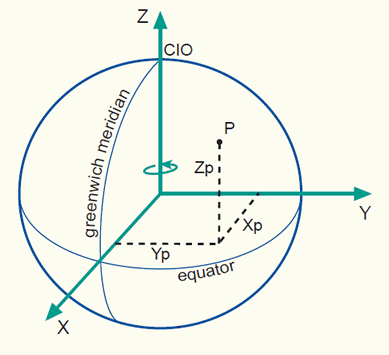
\includegraphics[width=0.7\textwidth]{coord_geocentric}
          \end{center}
          \caption[Sistema de coordenadas Geocentricas ]{Sistema de coordenadas Geocentricas, en la figura se muestra la posici\'on del punto P}
          \label{fig:coord_geocentric}
        \end{figure}

        Este Sistema de coordenadas no es muy usado en la representacion de datos.
        % , pero aveces se lo requiere para analisis de algoritmos y geometria computacional.
      % subsection coordenadas_geocentricas (end)  

      \subsection{Coordenadas Geograficas} % (fold)
      \label{sub:coordenadas_geograficas}
        Sistema de coordenadas Geográfico, utiliza las coordenadas angulares latitud  (phi o ${\phi}$) y longitud (lambda o ${\lambda}$). Este sistema de coordenadas se expresa en grados, se lo puede representar con la forma \emph{grados:minutos:segundos }\verb|(17° 23' 37.4226" S, 66° 8' 44.691" W)|, o de la forma mas comun \emph{grados decimales} \verb|(-66.1457475 S, -17.3937285 W)|.\\

        El sistema de coordenadas  mas amplimente usado, el que usan por defecto los sistemas GPS, es conocido como ``WGS 84'', y la mayoria de las aplicaciones que manejan mapas.\\

        \begin{figure}[!hbp]
          \begin{center}
            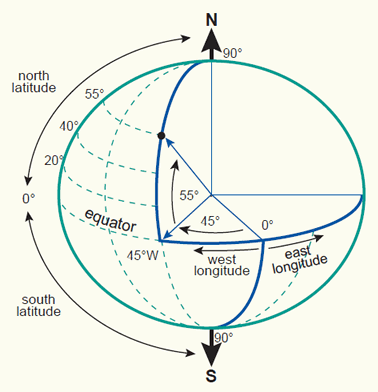
\includegraphics[width=0.7\textwidth]{coord_geographic}
          \end{center}
          \caption[Sistema de coordenadas Geográficos]{Sistema de coordenadas Geográficos, Es el sistema que maneja los mas amplimanete conocidos ``latitud y longitud''} 
          \label{fig:coord_geographic}
        \end{figure}   

      % subsection coordenadas_geograficas (end)

      \subsection{Coordenadas Proyectadas} % (fold)
      \label{sub:coordenadas_proyectadas}
        Un sistema de coordenadas proyectadas es una representación plana y bidimensional de la  tierra. Se basa en un sistema de coordenadas geográficas esf\'ericas, pero utiliza unidades de medida lineales para las coordenadas, de forma que los cálculos de distancia y área se pueden realizar en términos de esas mismas unidades.\cite{projected_ibm} \\

        Un sistema de coordenadas proyectadas requiere tomar la superficie esferica de la tierra y ``aplanarla'', este procedimiento se lo realiza con la finalidad de tener un mapa representable en una hoja de papel asi como en la pantalla de la computadora. Sin embargo este procedimiento introduce diversos tipos de distorci\'on por lo que existen diferentes clases de proyeciones que varian segun la region que se quiere representar de la Tierra.\\

        La proyecci\'on que usa Google Maps es la \textbf{Mercator Projection}, esta proyecci\'on esta dise\~nada para presevar los ángulos y las formas de las linias en forma recta, pero distorciona los tama\~nos y las distancias mientras mas lejos se encuentran de la linia del Ecuador. Esta proyecci\'on se puede apreciar en la figura \ref{fig:mercator_proyection}

        \begin{figure}[!hbp]
          \begin{center}
            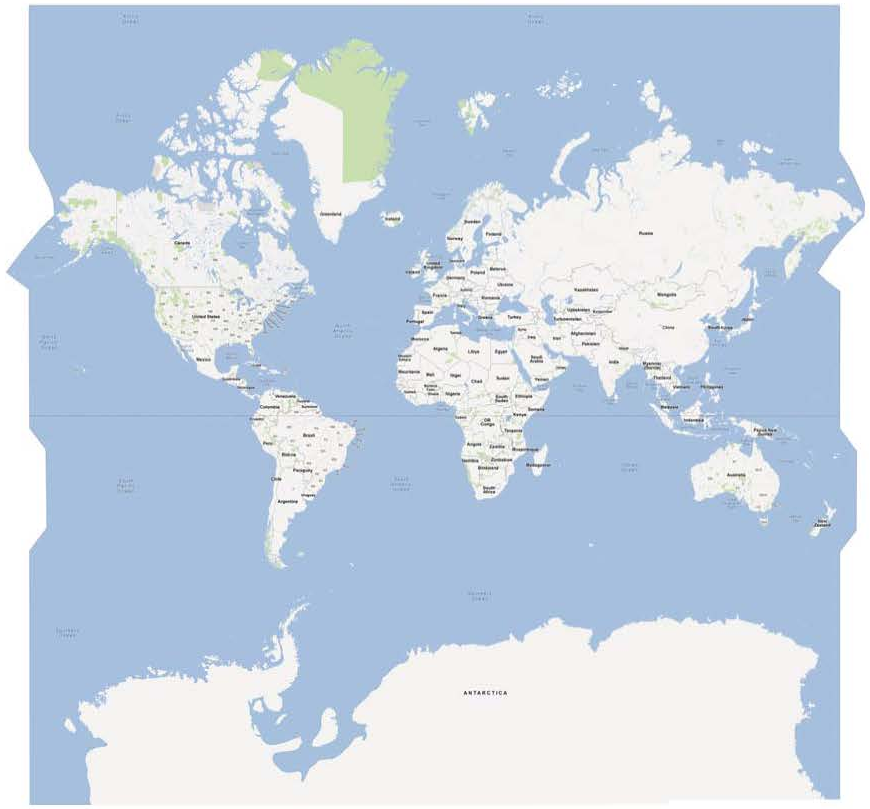
\includegraphics[width=0.6\textwidth]{mercator_proyection}
          \end{center}
          \caption[Sistema de coordenadas Proyectadas]{Google Maps usa la Proyección de Mercator para mostrar su mapa} 
          \label{fig:mercator_proyection}
        \end{figure}

        Tal como se puede apreciar en la figura \ref{fig:mercator_proyection}, la distorcion de esta proyecci\'on se hace evidente si se observa la zona de Groenlandia ya que pareceria tan grande como Africa o America del Sur, cosa que no es, ya que Groenlandia es casi 14 veces mas peque\~no que Africa. A pesar de esta distorci\'on tan marcada, la Proyección de Mercator es una de las mas usadas, de hecho Google Maps usa esta proyecci\'on.

      % subsection coordenadas_proyectadas (end)
  % section sistema_de_coordenadas_para_datos_geograficos (end)


  % \begin{description}
  %   % \item[SIG] Un Sistema de Informaci\'on Geografica es una manera de visualizar c\'omo es y que est\'a ocurriendo en algun lugar. La posibilidad de incorporar coordenadas con presici\'on.

  %   % A GIS is a colletion of software, normaly manipulatedby its user through a single interface, and designed to perform a wide range of operations on geographic data.  
  %   % Research  Methods in Geography
  %   % Basil Gomez and John Paul Jones III.
  %   % ISBN 978-1-4051-0710-5

  %   \item[Datum] 
  %   \item[] 
  %   \item[] 
  % \end{description}

  % procesar
  % Se tien
  % , Sistema de Posicionamiento Global por sus siglas en espa\~nol
% chapter geolocalizacion (end)

